\documentclass{article}\usepackage[]{graphicx}\usepackage[]{color}
%% maxwidth is the original width if it is less than linewidth
%% otherwise use linewidth (to make sure the graphics do not exceed the margin)
\makeatletter
\def\maxwidth{ %
  \ifdim\Gin@nat@width>\linewidth
    \linewidth
  \else
    \Gin@nat@width
  \fi
}
\makeatother

\definecolor{fgcolor}{rgb}{0.345, 0.345, 0.345}
\newcommand{\hlnum}[1]{\textcolor[rgb]{0.686,0.059,0.569}{#1}}%
\newcommand{\hlstr}[1]{\textcolor[rgb]{0.192,0.494,0.8}{#1}}%
\newcommand{\hlcom}[1]{\textcolor[rgb]{0.678,0.584,0.686}{\textit{#1}}}%
\newcommand{\hlopt}[1]{\textcolor[rgb]{0,0,0}{#1}}%
\newcommand{\hlstd}[1]{\textcolor[rgb]{0.345,0.345,0.345}{#1}}%
\newcommand{\hlkwa}[1]{\textcolor[rgb]{0.161,0.373,0.58}{\textbf{#1}}}%
\newcommand{\hlkwb}[1]{\textcolor[rgb]{0.69,0.353,0.396}{#1}}%
\newcommand{\hlkwc}[1]{\textcolor[rgb]{0.333,0.667,0.333}{#1}}%
\newcommand{\hlkwd}[1]{\textcolor[rgb]{0.737,0.353,0.396}{\textbf{#1}}}%
\let\hlipl\hlkwb

\usepackage{framed}
\makeatletter
\newenvironment{kframe}{%
 \def\at@end@of@kframe{}%
 \ifinner\ifhmode%
  \def\at@end@of@kframe{\end{minipage}}%
  \begin{minipage}{\columnwidth}%
 \fi\fi%
 \def\FrameCommand##1{\hskip\@totalleftmargin \hskip-\fboxsep
 \colorbox{shadecolor}{##1}\hskip-\fboxsep
     % There is no \\@totalrightmargin, so:
     \hskip-\linewidth \hskip-\@totalleftmargin \hskip\columnwidth}%
 \MakeFramed {\advance\hsize-\width
   \@totalleftmargin\z@ \linewidth\hsize
   \@setminipage}}%
 {\par\unskip\endMakeFramed%
 \at@end@of@kframe}
\makeatother

\definecolor{shadecolor}{rgb}{.97, .97, .97}
\definecolor{messagecolor}{rgb}{0, 0, 0}
\definecolor{warningcolor}{rgb}{1, 0, 1}
\definecolor{errorcolor}{rgb}{1, 0, 0}
\newenvironment{knitrout}{}{} % an empty environment to be redefined in TeX

\usepackage{alltt}

\usepackage{hyperref}
\usepackage[backend=bibtex, maxnames=10]{biblatex}
\usepackage{xargs}
\usepackage{xcolor}
\usepackage{soul}

\title{Package \textbf{CompSign}}
\author{Lena Morrill}
\date{October 2017}

\bibliography{../../CDA_in_Cancer/text/progress_text/bibliography.bib}

\newcommandx{\myemph}[2][1=]{\begin{center}\hl{#1}\end{center}}
\IfFileExists{upquote.sty}{\usepackage{upquote}}{}
\begin{document}

\maketitle

\textbf{CompSign} is a toolkit for the analysis of mutational signatures with an emphasis on the compositional analysis of exposures. An overview of the compositional nature of the exposures to mutational signatures, which has been often overlooked, is found elsewhere\footnote{cite myself}.

% The reference manual can be found \href{https://github.com/lm687/CompSign/blob/master/CompSign.pdf}{here}.

% \tableofcontents



\section{Installation}
\texttt{CompSign} can be installed as usual from github:

\begin{knitrout}
\definecolor{shadecolor}{rgb}{0.969, 0.969, 0.969}\color{fgcolor}\begin{kframe}
\begin{alltt}
\hlkwd{library}\hlstd{(devtools)}
\hlstd{devtools}\hlopt{::}\hlkwd{install_github}\hlstd{(}\hlstr{"lm687/CompSign"}\hlstd{)}
\end{alltt}
\end{kframe}
\end{knitrout}

\begin{knitrout}
\definecolor{shadecolor}{rgb}{0.969, 0.969, 0.969}\color{fgcolor}\begin{kframe}
\begin{alltt}
\hlkwd{library}\hlstd{(CompSign)}
\hlkwd{library}\hlstd{(compositions)}
\hlkwd{library}\hlstd{(MCMCpack)}      \hlcom{## for sampling from Dirichlet}
\hlkwd{library}\hlstd{(ggplot2)}
\end{alltt}
\end{kframe}
\end{knitrout}

\clearpage
\section{Datasets}
\begin{knitrout}
\definecolor{shadecolor}{rgb}{0.969, 0.969, 0.969}\color{fgcolor}\begin{kframe}
\begin{alltt}
\hlcom{## if the folder data/ is not in github}
\hlkwa{for}\hlstd{(i} \hlkwa{in} \hlkwd{list.files}\hlstd{(}\hlstr{"../data/"}\hlstd{,} \hlkwc{pattern} \hlstd{=} \hlstr{"*rda"}\hlstd{,} \hlkwc{full.names} \hlstd{=} \hlnum{TRUE}\hlstd{))\{}\hlkwd{load}\hlstd{(i)\}}
\end{alltt}
\end{kframe}
\end{knitrout}

The package contains several datasets of exposures to mutational signatures and metadata of the corresponding samples. These datasets are:
\begin{itemize}
\item SNV signatures
\begin{itemize}
\item Data for 560 breast cancer patients

\begin{knitrout}
\definecolor{shadecolor}{rgb}{0.969, 0.969, 0.969}\color{fgcolor}\begin{kframe}
\begin{alltt}
\hlcom{# data("Breast560")}
\hlstd{metadataBreast560} \hlkwb{<-} \hlkwd{metadata}\hlstd{(Breast560)}
\hlstd{exposuresBreast560} \hlkwb{<-} \hlkwd{count_matrix}\hlstd{(Breast560)}
\hlkwd{dim}\hlstd{(metadataBreast560);} \hlkwd{dim}\hlstd{(exposuresBreast560)}
\end{alltt}
\begin{verbatim}
## [1] 560  47
## [1] 560  12
\end{verbatim}
\end{kframe}
\end{knitrout}

\item Pan-cancer from EMu\cite{fischer2013emu} (cite dataset)
\end{itemize}
\item Copy Number signatures
\begin{itemize}
\item Ovarian cancer-derived signatures, as described in \cite{macintyre2018copy}. It contains data for 12k TCGA samples.

\begin{knitrout}
\definecolor{shadecolor}{rgb}{0.969, 0.969, 0.969}\color{fgcolor}\begin{kframe}
\begin{alltt}
\hlcom{#data("CNA_12K_TCGA")}
\hlstd{metadataCNA_12K_TCGA} \hlkwb{<-} \hlkwd{metadata}\hlstd{(CNA_12K_TCGA)}
\hlstd{exposuresCNA_12K_TCGA} \hlkwb{<-} \hlkwd{count_matrix}\hlstd{(CNA_12K_TCGA)}
\end{alltt}
\end{kframe}
\end{knitrout}

\item Pan-cancer copy number signatures
\end{itemize}
\item Synthetic data
\begin{knitrout}
\definecolor{shadecolor}{rgb}{0.969, 0.969, 0.969}\color{fgcolor}\begin{kframe}
\begin{alltt}
\hlkwd{dim}\hlstd{(}\hlkwd{metadata}\hlstd{(two_normal_pops))}
\end{alltt}
\begin{verbatim}
## [1] 2000    1
\end{verbatim}
\begin{alltt}
\hlkwd{dim}\hlstd{(}\hlkwd{count_matrix}\hlstd{(two_normal_pops))}
\end{alltt}
\begin{verbatim}
## [1] 2000    3
\end{verbatim}
\begin{alltt}
\hlcom{#data(two_normal_pops)}
\end{alltt}
\end{kframe}
\end{knitrout}
\end{itemize}

Data can be visualised as follows \hl{add this to the functions of the package}

\begin{knitrout}
\definecolor{shadecolor}{rgb}{0.969, 0.969, 0.969}\color{fgcolor}\begin{kframe}
\begin{alltt}
\hlkwd{source}\hlstd{(}\hlstr{"../../CDA_in_Cancer/code/functions/meretricious/pretty_plots/prettySignatures.R"}\hlstd{,} \hlkwc{print.eval} \hlstd{=} \hlnum{TRUE}\hlstd{)}
\hlkwd{createBarplot}\hlstd{(}\hlkwd{count_matrix}\hlstd{(Breast560),} \hlkwc{remove_labels} \hlstd{=} \hlnum{TRUE}\hlstd{,}
              \hlkwc{order} \hlstd{=} \hlkwd{names}\hlstd{(}\hlkwd{sort}\hlstd{(}\hlkwd{count_matrix}\hlstd{(Breast560)[,}\hlnum{1}\hlstd{])))}
\end{alltt}
\begin{verbatim}
## Creating plot... it might take some time if the data are large. Number of samples: 560
\end{verbatim}
\end{kframe}
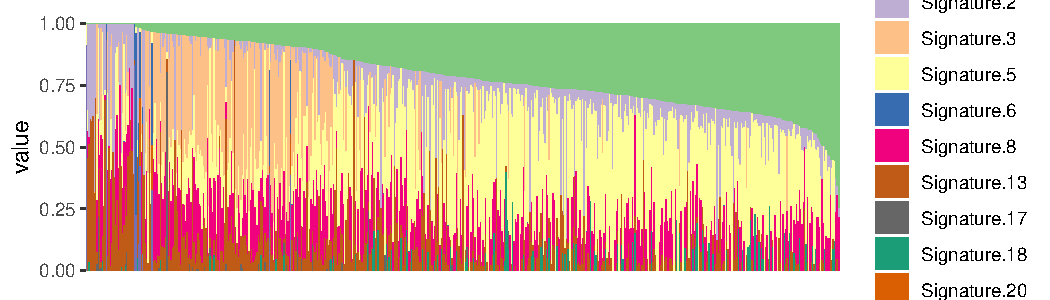
\includegraphics[width=\maxwidth]{figure/unnamed-chunk-8-1} 

\end{knitrout}


\section{Create a \texttt{CompSign} object}
This is a minimal example for transforming a matrix into a \emph{sign} object
\begin{knitrout}
\definecolor{shadecolor}{rgb}{0.969, 0.969, 0.969}\color{fgcolor}\begin{kframe}
\begin{alltt}
\hlstd{basic_matrix} \hlkwb{<-} \hlkwd{matrix}\hlstd{(}\hlkwd{runif}\hlstd{(}\hlnum{12}\hlstd{),} \hlkwc{nrow} \hlstd{=} \hlnum{4}\hlstd{)}
\hlkwd{colnames}\hlstd{(basic_matrix)} \hlkwb{<-} \hlkwd{paste0}\hlstd{(}\hlstr{'s'}\hlstd{,} \hlnum{1}\hlopt{:}\hlnum{3}\hlstd{)}
\hlkwd{rownames}\hlstd{(basic_matrix)} \hlkwb{<-} \hlkwd{paste0}\hlstd{(}\hlstr{'Sample '}\hlstd{,} \hlnum{1}\hlopt{:}\hlnum{4}\hlstd{)}
\hlstd{basic_sign} \hlkwb{<-} \hlkwd{to_sign}\hlstd{(basic_matrix)}
\hlstd{basic_sign}
\end{alltt}
\begin{verbatim}
## An object of class "sign"
## Slot "id":
## [1] "basic_matrix"
## 
## Slot "id_samples":
## [1] "Sample 1" "Sample 2" "Sample 3" "Sample 4"
## 
## Slot "id_signatures":
## [1] "s1" "s2" "s3"
## 
## Slot "count_matrix":
##                 s1         s2        s3
## Sample 1 0.4518026 0.16322933 0.6123104
## Sample 2 0.7720006 0.98059998 0.2178652
## Sample 3 0.5882031 0.72776198 0.7582357
## Sample 4 0.5280328 0.08958892 0.3338896
## 
## Slot "modified":
## [1] FALSE
\end{verbatim}
\end{kframe}
\end{knitrout}

A \emph{sign} object can be summarised as follows:

\hl{add\_together\_matrix?? what is this?}

\begin{knitrout}
\definecolor{shadecolor}{rgb}{0.969, 0.969, 0.969}\color{fgcolor}\begin{kframe}
\begin{alltt}
\hlstd{results_sumarise} \hlkwb{<-} \hlkwd{summarise}\hlstd{(}\hlkwd{add_together_matrix}\hlstd{(basic_sign))}
\hlstd{results_sumarise}
\end{alltt}
\begin{verbatim}
## $General
## [1] "Object of class sign"
## 
## $`Number of signatures`
## [1] 3
## 
## $`Number of samples`
## [1] 4
## 
## $`Geometric means of signatures`
##        s1        s3        s2 
## 0.5737050 0.4286883 0.3196196 
## 
## $Covariance
##             s1          s2          s3
## s1  0.01865543  0.05294645 -0.01914269
## s2  0.05294645  0.18810895 -0.01572702
## s3 -0.01914269 -0.01572702  0.06166089
\end{verbatim}
\end{kframe}
\end{knitrout}

\clearpage
\section{Battery of tests}
This section takes largely from Aitchison's pioneering work\cite{aitchison1982statistical} and its succession\cite{pawlowsky2015modeling}.

\subsection{Test for normality}
\begin{knitrout}
\definecolor{shadecolor}{rgb}{0.969, 0.969, 0.969}\color{fgcolor}\begin{kframe}
\begin{alltt}
\hlkwd{par}\hlstd{(}\hlkwc{mfrow}\hlstd{=}\hlkwd{c}\hlstd{(}\hlnum{1}\hlstd{,}\hlnum{2}\hlstd{))}
\hlkwd{qqnorm.acomp}\hlstd{(}\hlkwd{acomp}\hlstd{(two_normal_pops}\hlopt{@}\hlkwc{count_matrix}\hlstd{),} \hlkwc{pch}\hlstd{=}\hlnum{19}\hlstd{,} \hlkwc{cex}\hlstd{=}\hlnum{0.2}\hlstd{)}
\end{alltt}
\end{kframe}
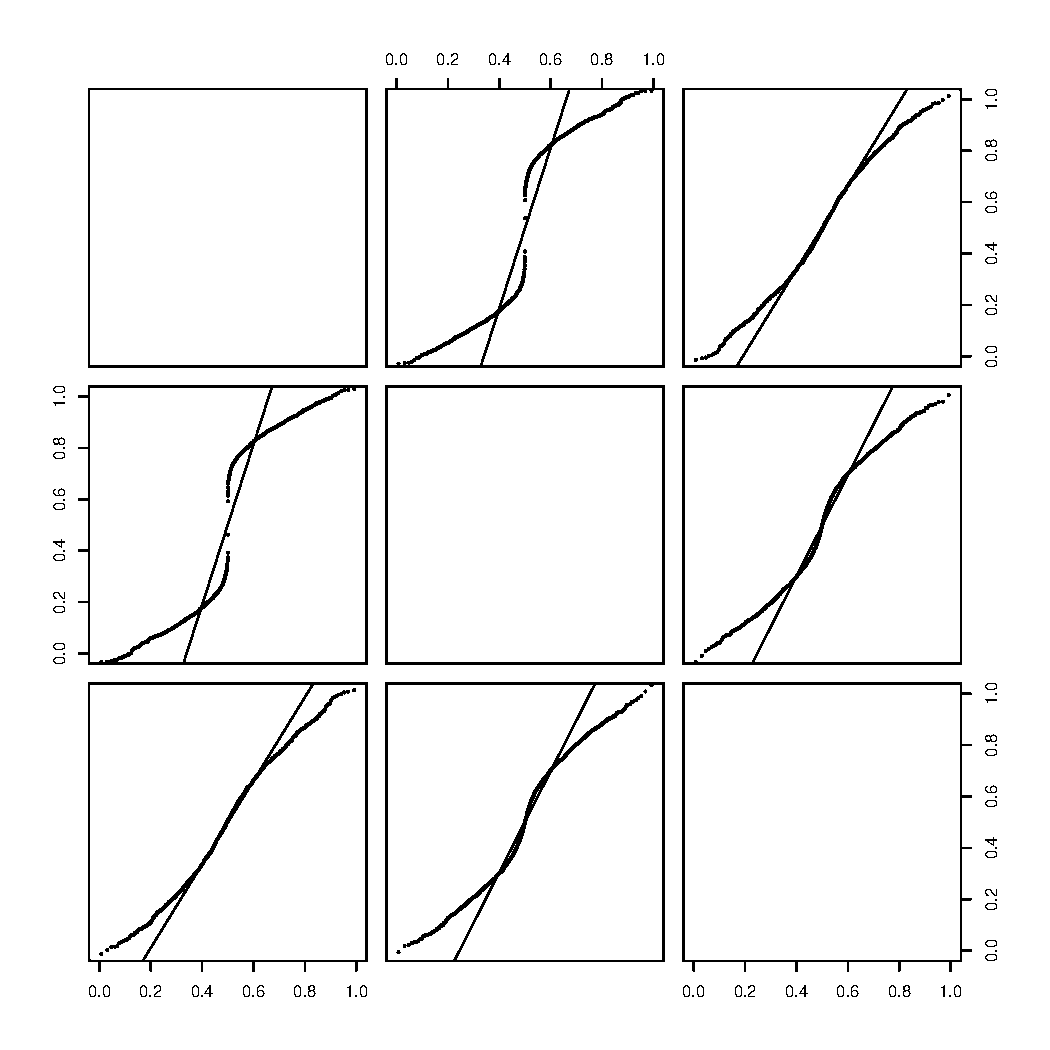
\includegraphics[width=\maxwidth]{figure/unnamed-chunk-11-1} 
\begin{kframe}\begin{alltt}
\hlkwd{qqnorm.acomp}\hlstd{(}\hlkwd{acomp}\hlstd{(two_normal_pops}\hlopt{@}\hlkwc{count_matrix}\hlstd{[}\hlnum{1}\hlopt{:}\hlnum{1000}\hlstd{,]),} \hlkwc{pch}\hlstd{=}\hlnum{19}\hlstd{,} \hlkwc{cex}\hlstd{=}\hlnum{0.2}\hlstd{)}
\end{alltt}
\end{kframe}
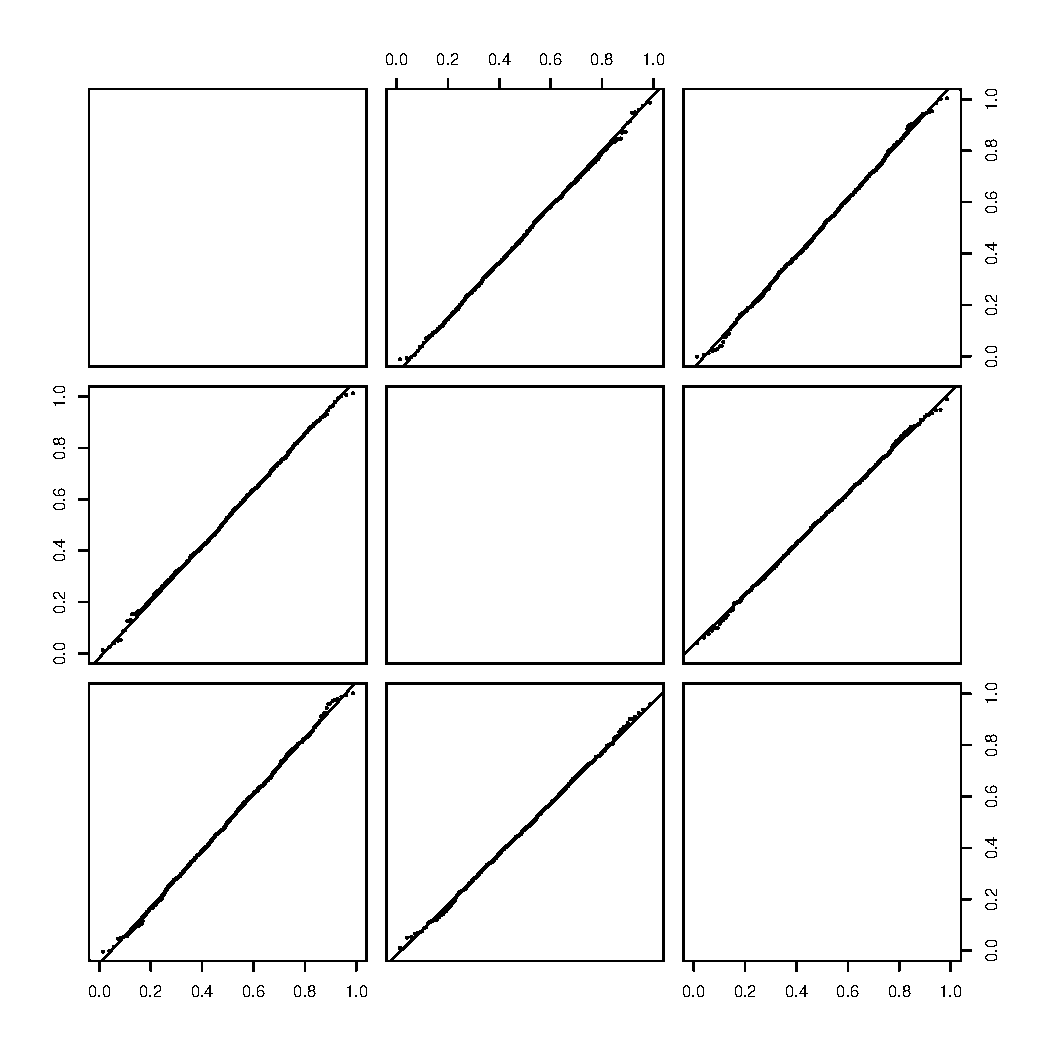
\includegraphics[width=\maxwidth]{figure/unnamed-chunk-11-2} 

\end{knitrout}

\subsection{Test for equality}
Test for equality of means.
\begin{knitrout}
\definecolor{shadecolor}{rgb}{0.969, 0.969, 0.969}\color{fgcolor}\begin{kframe}
\begin{alltt}
\hlkwd{compare_populations}\hlstd{(}\hlkwc{predictors} \hlstd{=} \hlkwd{count_matrix}\hlstd{(Breast560),}
                    \hlkwc{response} \hlstd{=} \hlkwd{as.numeric}\hlstd{(}\hlkwd{as.factor}\hlstd{(}\hlkwd{metadata}\hlstd{(Breast560)}\hlopt{$}\hlstd{final.ER)))}
\end{alltt}
\begin{verbatim}
## $note
## [1] "James test"
## 
## $mesoi
##                  X1         X2       X3           X4        X5       X6
## Sample 1 -1.6969917 -0.9470633 1.923296 -0.103998542 0.2707288 1.528197
## Sample 2  0.8022291 -3.6033765 2.143807  0.002721535 0.6369184 1.607875
##                X7       X8       X9      X10
## Sample 1 1.271388 1.248926 1.016479 1.017358
## Sample 2 1.086473 1.283400 1.083742 1.048809
## 
## $info
##               test            p-value         correction 
##       2.359067e+02       5.324172e-43       1.042820e+00 
## corrected.critical 
##       1.909095e+01
\end{verbatim}
\end{kframe}
\end{knitrout}





\section{Clustering of samples}
Samples can simply be clustered by the cosine similarity of their exposures, as done in Ren et al.

\begin{knitrout}
\definecolor{shadecolor}{rgb}{0.969, 0.969, 0.969}\color{fgcolor}\begin{kframe}
\begin{alltt}
\hlstd{res_outerCosineSimilaritySNV} \hlkwb{<-} \hlkwd{outerCosineSimilarity}\hlstd{(exposuresBreast560, exposuresBreast560,} \hlkwc{verbose}\hlstd{=}\hlnum{FALSE}\hlstd{)}
\end{alltt}
\begin{verbatim}
## [1] 560  12
## [1] 560  12
\end{verbatim}
\begin{alltt}
\hlstd{ComplexHeatmap}\hlopt{::}\hlkwd{Heatmap}\hlstd{(res_outerCosineSimilaritySNV)}
\end{alltt}
\end{kframe}
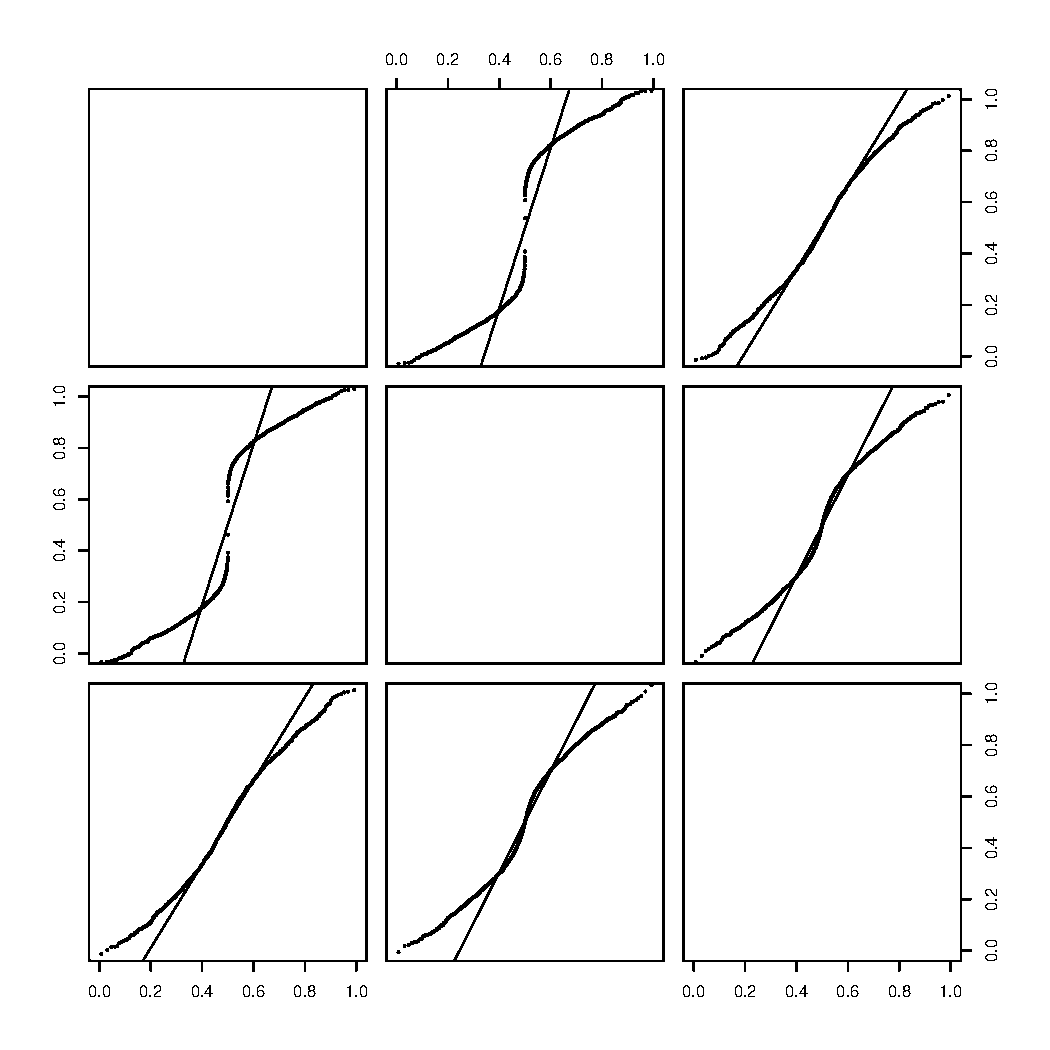
\includegraphics[width=\maxwidth]{figure/unnamed-chunk-14-1} 
\begin{kframe}\begin{alltt}
\hlcom{# res_outerCosineSimilarityCNA <- outerCosineSimilarity(exposuresCNA_12K_TCGA[metadataCNA_12K_TCGA$project_id %in% c("TCGA-BRCA", "TCGA-SKCM"),],}
\hlcom{#                                                       exposuresCNA_12K_TCGA[metadataCNA_12K_TCGA$project_id %in% c("TCGA-BRCA", "TCGA-SKCM"),],}
\hlcom{#                                                       verbose=FALSE)}
\hlcom{# ComplexHeatmap::Heatmap(res_outerCosineSimilarityCNA)}
\end{alltt}
\end{kframe}
\end{knitrout}

\clearpage

\clearpage
\printbibliography

\clearpage
\section{Session info}
\begin{knitrout}
\definecolor{shadecolor}{rgb}{0.969, 0.969, 0.969}\color{fgcolor}\begin{kframe}
\begin{alltt}
  \hlkwd{sessionInfo}\hlstd{()}
\end{alltt}
\begin{verbatim}
## R version 3.5.1 (2018-07-02)
## Platform: x86_64-apple-darwin15.6.0 (64-bit)
## Running under: macOS  10.14.4
## 
## Matrix products: default
## BLAS: /Library/Frameworks/R.framework/Versions/3.5/Resources/lib/libRblas.0.dylib
## LAPACK: /Library/Frameworks/R.framework/Versions/3.5/Resources/lib/libRlapack.dylib
## 
## locale:
## [1] C/zh_CN.UTF-8/C/C/C/C
## 
## attached base packages:
## [1] stats     graphics  grDevices utils     datasets  methods   base     
## 
## other attached packages:
##  [1] Compositional_3.4   RColorBrewer_1.1-2  reshape2_1.4.3     
##  [4] ggthemr_1.1.0       ggplot2_3.1.1       MCMCpack_1.4-4     
##  [7] MASS_7.3-51.4       coda_0.19-2         compositions_1.40-2
## [10] bayesm_3.1-1        energy_1.7-5        robustbase_0.93-4  
## [13] tensorA_0.36.1      CompSign_0.1.0      knitr_1.22         
## 
## loaded via a namespace (and not attached):
##  [1] Rcpp_1.0.1         lattice_0.20-38    assertthat_0.2.1  
##  [4] digest_0.6.18      foreach_1.4.4      R6_2.4.0          
##  [7] plyr_1.8.4         MatrixModels_0.4-1 RcppZiggurat_0.1.5
## [10] stats4_3.5.1       evaluate_0.13      spam_2.2-2        
## [13] highr_0.8          pillar_1.3.1       rlang_0.3.4       
## [16] lazyeval_0.2.2     SparseM_1.77       Matrix_1.2-17     
## [19] labeling_0.3       stringr_1.4.0      emplik_1.0-4.3    
## [22] munsell_0.5.0      compiler_3.5.1     numDeriv_2016.8-1 
## [25] xfun_0.6           pkgconfig_2.0.2    mnormt_1.5-5      
## [28] mcmc_0.9-6         tidyselect_0.2.5   tibble_2.1.1      
## [31] codetools_0.2-16   crayon_1.3.4       dplyr_0.8.0.1     
## [34] withr_2.1.2        grid_3.5.1         gtable_0.3.0      
## [37] magrittr_1.5       scales_1.0.0       Rfast_1.9.3       
## [40] stringi_1.4.3      sn_1.5-3           doParallel_1.0.14 
## [43] boot_1.3-22        iterators_1.0.10   tools_3.5.1       
## [46] glue_1.3.1         DEoptimR_1.0-8     purrr_0.3.2       
## [49] maps_3.3.0         fields_9.7         parallel_3.5.1    
## [52] mixture_1.5        colorspace_1.4-1   dotCall64_1.0-0   
## [55] quantreg_5.38
\end{verbatim}
\end{kframe}
\end{knitrout}


\section{Optimal selection of partition}

\begin{knitrout}
\definecolor{shadecolor}{rgb}{0.969, 0.969, 0.969}\color{fgcolor}\begin{kframe}
\begin{alltt}
\hlkwd{set.seed}\hlstd{(}\hlnum{1234}\hlstd{)}

\hlcom{## simulated data}
\hlstd{Nsig} \hlkwb{<-} \hlnum{5}\hlstd{; Nsamp} \hlkwb{<-} \hlnum{100}
\hlstd{props} \hlkwb{<-} \hlstd{MCMCpack}\hlopt{::}\hlkwd{rdirichlet}\hlstd{(Nsamp,} \hlkwd{c}\hlstd{(}\hlkwd{rep}\hlstd{(}\hlnum{1}\hlstd{,Nsig)))}
\hlkwd{colnames}\hlstd{(props)} \hlkwb{<-} \hlkwd{paste0}\hlstd{(}\hlstr{'Sig'}\hlstd{,} \hlnum{1}\hlopt{:}\hlstd{Nsig)}
\hlkwd{rownames}\hlstd{(props)} \hlkwb{<-} \hlkwd{paste0}\hlstd{(}\hlstr{'Sam '}\hlstd{,} \hlnum{1}\hlopt{:}\hlstd{Nsamp)}
\hlcom{## increase exposure to signature 1 in the first}
\hlcom{## Nsamp/2, and re-normalise (two groups)}
\hlstd{props[}\hlnum{1}\hlopt{:}\hlkwd{floor}\hlstd{(Nsamp}\hlopt{/}\hlnum{2}\hlstd{),} \hlnum{1}\hlstd{]} \hlkwb{<-} \hlstd{props[}\hlnum{1}\hlopt{:}\hlkwd{floor}\hlstd{(Nsamp}\hlopt{/}\hlnum{2}\hlstd{),} \hlnum{1}\hlstd{]} \hlopt{+} \hlnum{1.5}
\hlstd{props} \hlkwb{<-} \hlkwd{sweep}\hlstd{(props,} \hlnum{1}\hlstd{,} \hlkwd{rowSums}\hlstd{(props),} \hlstr{'/'}\hlstd{)}
\hlkwd{createBarplot}\hlstd{(props,} \hlkwc{remove_labels} \hlstd{=} \hlnum{TRUE}\hlstd{)}
\end{alltt}
\begin{verbatim}
## Creating plot... it might take some time if the data are large. Number of samples: 100
\end{verbatim}
\end{kframe}
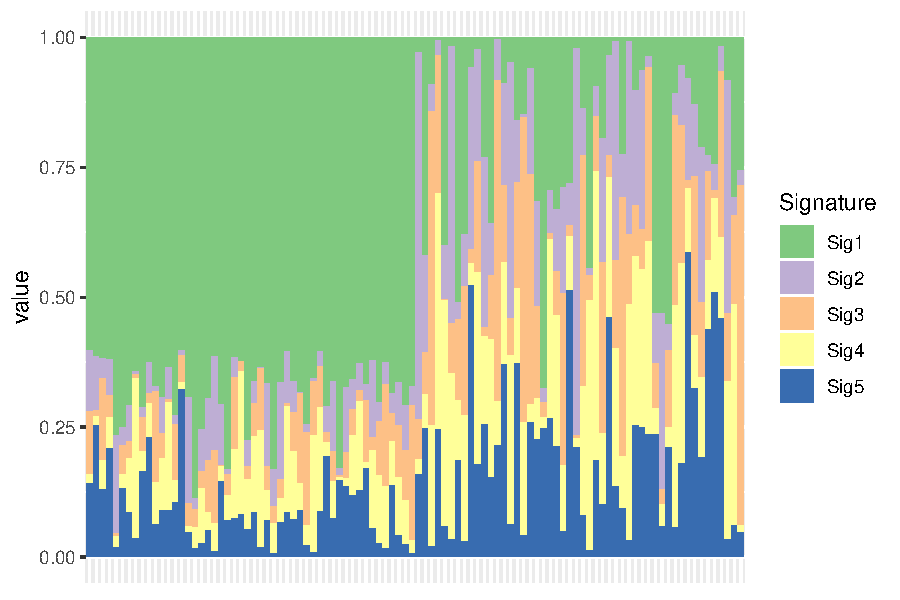
\includegraphics[width=\maxwidth]{figure/unnamed-chunk-16-1} 
\begin{kframe}\begin{alltt}
\hlcom{## corresponds to partitioning as follows:}
\hlcom{##(s1, s2, s3) vs (s4, s5)}
\hlstd{V} \hlkwb{<-} \hlkwd{c}\hlstd{(}\hlnum{1}\hlstd{,} \hlnum{1}\hlstd{,} \hlnum{1}\hlstd{,} \hlopt{-}\hlnum{1}\hlstd{,} \hlopt{-}\hlnum{1}\hlstd{)}
\hlcom{# plot(density(ilr(props, V = V)))}
\hlkwd{boxplot}\hlstd{(}\hlkwd{ilr}\hlstd{(props,} \hlkwc{V} \hlstd{= V)[}\hlnum{1}\hlopt{:}\hlkwd{floor}\hlstd{(Nsamp}\hlopt{/}\hlnum{2}\hlstd{)],}
        \hlkwd{ilr}\hlstd{(props,} \hlkwc{V} \hlstd{= V)[(}\hlkwd{floor}\hlstd{(Nsamp}\hlopt{/}\hlnum{2}\hlstd{)}\hlopt{+}\hlnum{1}\hlstd{)}\hlopt{:}\hlstd{Nsamp],} \hlkwc{main} \hlstd{=} \hlstr{'Comparison of ilr of (s1, s2, s3) vs (s4, s5) for the two groups'}\hlstd{)}
\end{alltt}
\end{kframe}
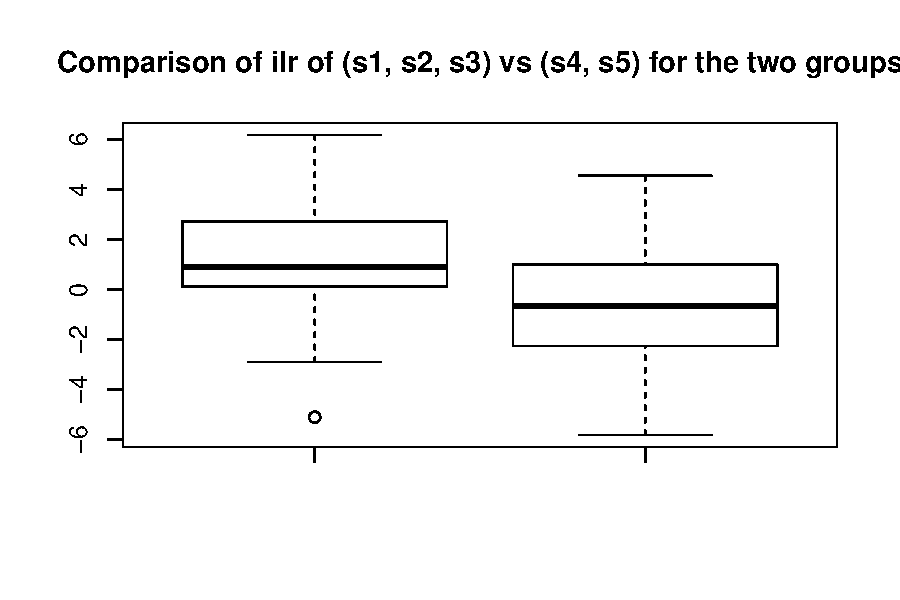
\includegraphics[width=\maxwidth]{figure/unnamed-chunk-16-2} 
\begin{kframe}\begin{alltt}
\hlkwd{t.test}\hlstd{(}\hlkwd{ilr}\hlstd{(props,} \hlkwc{V} \hlstd{= V)[}\hlnum{1}\hlopt{:}\hlkwd{floor}\hlstd{(Nsamp}\hlopt{/}\hlnum{2}\hlstd{)],}
       \hlkwd{ilr}\hlstd{(props,} \hlkwc{V} \hlstd{= V)[(}\hlkwd{floor}\hlstd{(Nsamp}\hlopt{/}\hlnum{2}\hlstd{)}\hlopt{+}\hlnum{1}\hlstd{)}\hlopt{:}\hlstd{Nsamp])}\hlopt{$}\hlstd{p.value}
\end{alltt}
\begin{verbatim}
## [1] 8.913039e-06
\end{verbatim}
\begin{alltt}
\hlstd{it_partitions} \hlkwb{<-} \hlkwd{c}\hlstd{()}
\hlkwa{if}\hlstd{(Nsig} \hlopt{>} \hlnum{8}\hlstd{)\{}\hlkwd{warning}\hlstd{(}\hlstr{'Large number of signatures'}\hlstd{)\}}
\hlkwa{for}\hlstd{(k} \hlkwa{in} \hlnum{1}\hlopt{:}\hlkwd{floor}\hlstd{(Nsig}\hlopt{/}\hlnum{2}\hlstd{))\{}
  \hlstd{it_partitions} \hlkwb{<-} \hlkwd{c}\hlstd{(it_partitions,} \hlkwd{lapply}\hlstd{(}\hlnum{1}\hlopt{:}\hlkwd{ncol}\hlstd{(}\hlkwd{combn}\hlstd{(}\hlnum{1}\hlopt{:}\hlstd{Nsig, k)),} \hlkwa{function}\hlstd{(}\hlkwc{x}\hlstd{)} \hlkwd{combn}\hlstd{(}\hlnum{1}\hlopt{:}\hlstd{Nsig, k)[,x]))}
\hlstd{\}}
\hlstd{pvals} \hlkwb{<-} \hlkwd{rep}\hlstd{(}\hlnum{NA}\hlstd{,} \hlkwd{length}\hlstd{(it_partitions))}
\hlstd{ict} \hlkwb{<-} \hlnum{1}
\hlkwa{for}\hlstd{(i} \hlkwa{in} \hlstd{it_partitions)\{}
  \hlstd{V} \hlkwb{<-} \hlkwd{rep}\hlstd{(}\hlopt{-}\hlnum{1}\hlstd{, Nsig)}
  \hlstd{V[i]} \hlkwb{<-} \hlnum{1}
  \hlstd{pvals[ict]} \hlkwb{<-} \hlkwd{t.test}\hlstd{(}\hlkwd{ilr}\hlstd{(props,} \hlkwc{V} \hlstd{= V)[}\hlnum{1}\hlopt{:}\hlkwd{floor}\hlstd{(Nsamp}\hlopt{/}\hlnum{2}\hlstd{)],}
         \hlkwd{ilr}\hlstd{(props,} \hlkwc{V} \hlstd{= V)[(}\hlkwd{floor}\hlstd{(Nsamp}\hlopt{/}\hlnum{2}\hlstd{)}\hlopt{+}\hlnum{1}\hlstd{)}\hlopt{:}\hlstd{Nsamp])}\hlopt{$}\hlstd{p.value}
  \hlstd{ict} \hlkwb{<-} \hlstd{ict} \hlopt{+} \hlnum{1}
\hlstd{\}}

\hlstd{groups} \hlkwb{<-} \hlkwd{sapply}\hlstd{(it_partitions, paste0,} \hlkwc{collapse}\hlstd{=}\hlstr{'_'}\hlstd{)}
\hlkwd{ggplot}\hlstd{(}\hlkwd{data.frame}\hlstd{(}\hlkwc{pval}\hlstd{=pvals,} \hlkwc{group}\hlstd{=groups),}
       \hlkwd{aes}\hlstd{(}\hlkwc{x}\hlstd{=}\hlkwd{factor}\hlstd{(group,} \hlkwc{levels}\hlstd{=groups[}\hlkwd{order}\hlstd{(pvals)]),} \hlkwc{y}\hlstd{=}\hlkwd{log}\hlstd{(pval)))}\hlopt{+}
  \hlkwd{geom_point}\hlstd{()} \hlopt{+} \hlkwd{ggtitle}\hlstd{(}\hlstr{'P value for comparing a group (x-axis)\textbackslash{}nto its complementary'}\hlstd{)}\hlopt{+}
  \hlkwd{labs}\hlstd{(}\hlkwc{x}\hlstd{=}\hlstr{'Group'}\hlstd{)}
\end{alltt}
\end{kframe}
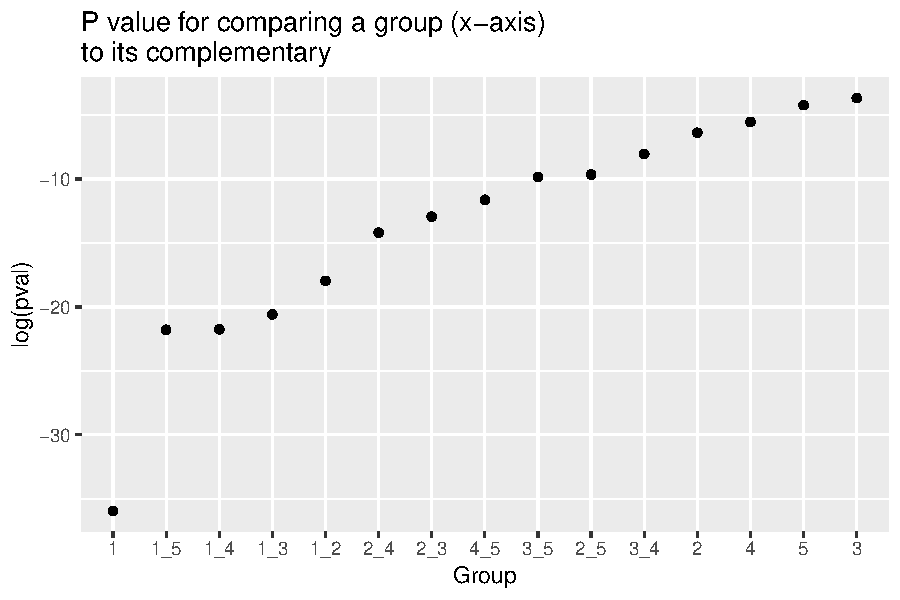
\includegraphics[width=\maxwidth]{figure/unnamed-chunk-16-3} 
\begin{kframe}\begin{alltt}
\hlcom{##' We expected 1 to be the one with lowest p-val}
\hlcom{##' as this is how we created the dataset.}
\hlcom{##' Groups containing signature 1 follow.}
\end{alltt}
\end{kframe}
\end{knitrout}

\end{document}
%
% \section{Linear model for numerical predictors}
% <<>>=
% ## This chunk was last ran in
% timestamp()
%
% tmp_merged_compositional <- new("merged_compositional",
%                                 id='adas',
%                                 id_samples=paste0("sam", 1:30),
%                                 id_signatures= c('s1', 's2', 's3', 's4'), ## signature names
%                                 count_matrix=MCMCpack::rdirichlet(30, c(1,1,1,1)),
%                                 df=data.frame(a=sample(1:1e4, 30), b=rep(10, 30)))
% comp_lm(tmp_merged_compositional)
% @
%
% \section{Importing data}
% <<>>=
% ## This chunk was last ran in
% timestamp()
%
% biplot(princomp(acomp(MCMCpack::rdirichlet(30, rep(1, 4)))))
%
% @
%
% \subsection{Testing hypotheses about two populations}
% We might have our samples split into two categories; e.g. sex. As in Aithison 1986\cite{}, I follow a hierarchy of alternative hypotheses, from least to most complex.
%
% Our first question is whether two populations have the same covariance and structure and center (i.e. if there is any distributional difference)
%
% <<>>=
% ## This chunk was last ran in
% timestamp()
% ##TODO!!
% @
%
% The next is whether the populations have a different center:
%
% <<>>=
% ## This chunk was last ran in
% timestamp()
% ## This dataset includes the two components above, as well as four others
% ## (a total of seven)
% data("two_normal_pops_extended")
%
% ## Data from the Landscape... paper
% data("Breast560")
%
% wrapper_compare_populations <- function(predictors, response, ...){
%   if(length(unique(response)) == 2){
%     tmp <- compare_populations(predictors, response, ...)
%     tmp <- tmp$info[1:2]
%     tmp
%   }
% }
%
% x <- do.call('rbind', lapply(1:ncol(metadata(Breast560)),
%        function(k){
%          wrapper_compare_populations(predictors = count_matrix(Breast560),
%                                      response = metadata(Breast560)[,k])
%          }
%        ))
%
%
% x
%
% @
%
%
% Not sure if this is correct
% <<fig.width=3.5,fig.height=5>>=
% source("../../CDA_in_Cancer/code/functions/basic_functions.R")
% plotPCA(ilr(count_matrix(Breast560)), pch=4, col='blue')
% @
%
%
% \section{Battery of tests}
%
%
% \subsection{Logistic regression}
% Based on ACDWR pg 200
%
% <<>>=
% #setwd("~/Documents/PhD/CompSign/vignette_knitr/")
% load("../data/two_normal_pops_extended.rda")
% load("../data/two_normal_pops_extended.rda")
% load("../data/CNA_12K_TCGA.rda")
%
% ## avoid perfect separation
% L <- length((as.numeric(metadata(two_normal_pops_extended)[,1])))
% scramble <- sample(1:L, floor(L*0.05), replace = FALSE)
%
% scrambled_labels <- (as.numeric(metadata(two_normal_pops_extended)[,1]))
% scrambled_labels[scramble] <- 1-scrambled_labels[scramble]
%
% auxcomp <- scale(ilr(count_matrix(two_normal_pops_extended)),
%                  center = TRUE, scale = FALSE)
%
% summary(glm(formula = scrambled_labels ~ ilr(acomp(count_matrix(two_normal_pops_extended))),
%             family = binomial(link = "logit")))
%
% res <- comp_logistic(count_matrix(two_normal_pops), scrambled_labels)
% res
%
% resB <- comp_logistic(count_matrix(two_normal_pops_extended), scrambled_labels)
% resB
%
% resCNA_gender <- comp_logistic(count_matrix(cleanObject(CNA_12K_TCGA, 'gender')),
%                               metadata(cleanObject(CNA_12K_TCGA, 'gender'))[,'gender'])
% resCNA_gender
%
% ## below: incorrect
% resCNA_race <- comp_logistic(count_matrix(cleanObject(CNA_12K_TCGA, 'race')),
%                               metadata(cleanObject(CNA_12K_TCGA, 'race'))[,'race'], relax_binary_assumption = TRUE)
%
% resCNA_race
%
% @
%
% With data from 560 BRCA:
%
% <<>>=
% load("../data/Breast560.rda")
%
% resBRCA_finalER <- comp_logistic(count_matrix(cleanObject(Breast560, 'final.ER')),
%                               metadata(cleanObject(Breast560, 'final.ER'))[,'final.ER'])
% resBRCA_finalER
% resBRCA_finalPR <- comp_logistic(count_matrix(cleanObject(Breast560, 'final.PR')),
%                                  metadata(cleanObject(Breast560, 'final.PR'))[,'final.PR'])
% resBRCA_finalPR
% @
%
% How to get p-values? I don't think the below is correct
% <<>>=
% give_pval <- function(summary_obj){
%   z <- summary_obj$coefficients/summary_obj$standard.errors
%   # 2-tailed Wald z tests to test significance of coefficients
%   p <- (1 - pnorm(abs(z), 0, 1)) * 2
%   p
% }
%
% give_pval(res$summary)             ## 1 and two are; the third one too (higher p-val) (third one wasn't expected, as far as I know?)
% give_pval(resB$summary)            ## 1 and two are; the rest are not (as expected)
% give_pval(resCNA_gender$summary)   ## are are statistically significant for the copy number signatures
% give_pval(resBRCA_finalER$summary) ## signature 1 significant
% give_pval(resBRCA_finalPR$summary) ## none are statistically significant
% give_pval(resCNA_race$summary)     ## some statistically significant
% @
%
% <<>>=
% wrapper_single_logReg <- function(colname, Ddd){
%     print('asdsd2')
%     print(head(metadata((Ddd))))
%     Ddd <- cleanObject(Ddd, colname)
%     compData = count_matrix(Ddd)
%     binaryLabels = metadata(Ddd)[,colname]
%
%     tmp <- comp_logistic(compData = compData,
%                          binaryLabels = binaryLabels,
%                          relax_binary_assumption = TRUE)
% #    give_pval(tmp$summary)
%     print(give_pval(tmp$summary))
%     cbind.data.frame(rep(colname, nrow( give_pval(tmp$summary))), give_pval(tmp$summary))
%     cbind.data.frame(rep(colname, nrow( give_pval(tmp$summary))), give_pval(tmp$summary))
% }
% wrapper_multiple_logReg <- function(dataset, colnames){
%   print('asdsd')
%   head(metadata(dataset))
%   do.call('rbind', lapply(colnames, function(X) wrapper_single_logReg(colname = X, Ddd = dataset)))
% }
%
% wrapper_single_logReg('race', CNA_12K_TCGA)
% all_cna <- wrapper_multiple_logReg(dataset = CNA_12K_TCGA,
%                                  colnames = c('race', 'ethnicity', 'gender', 'alcohol_history'))
%
% all_cna_coefs <- lapply(c('race', 'ethnicity', 'gender', 'alcohol_history'), function(lab){
%   comp_logistic(compData = count_matrix(cleanObject(CNA_12K_TCGA)),
%                 binaryLabels = metadata(cleanObject(CNA_12K_TCGA))[,lab],
%                 relax_binary_assumption = TRUE)
%   })
% ## cont...
%
% ## 'tissue_or_organ_of_origin':  too many (1260) weights
%
% library(pheatmap)
% source("../../CDA_in_Cancer/code/functions/WrapperlikeFunctions.R")
% pheatmap0(all_cna[,-1], nonames = FALSE, annotation_row = data.frame(all_cna[,1], row.names = rownames(all_cna[,-1])))
% @
%
% <<>>=
% require(reshape2)
% require(ggplot2)
% molten_pvals <- melt(all_cna)
% colnames(molten_pvals) <- c('variable', 'signature', 'value')
% ggplot(molten_pvals, aes(x=interaction(variable,signature), y=-log(value), col=signature))+
%   geom_point()+
%   geom_hline(aes(yintercept=-log(0.05)))
%
%
% ## if I want a sort of volcano plot I need the coefs (continue all_cna_coefs)
%
% @
%
